%% Sect. 1 -- from augur_AMT_§1 draft v1 (2026-09-21); research questions and restructuring 2026-09-29.
\introduction
\label{sec:1}

A DOAS retrieval returns more than a concentration. It returns a residual, a chi-square, a parameter covariance and a
convergence flag, and these travel with the concentration into averaging, filtering, trend fits and comparisons with
models and other instruments. They are read as a statement of trust: a small residual means the model described the spectrum, a converged flag
means the optimiser found the answer, and the reported 1$\sigma$ means the concentration is known that well. Each reading is conditional, and the conditions are not reported
alongside the numbers.

This paper asks two questions about that gap. First, how large are the errors that a fit report cannot see, when they
are measured by perturbing the calibration chain and re-running the retrieval? Second, what information does the
pipeline already hold, and discard, that would flag a failed retrieval? A third category emerges from the answers:
errors that neither the fit report nor any of the fields we propose can detect (Sect.~\ref{sec:6.5}).

The first question has a partial answer in the DOAS literature. The uncertainty a DOAS fit reports is the propagation
of the residual scatter through the linear system, and it is correct only if the residual is white and the forward
model complete. \citet{Stutz_1996} showed that structure in the residual inflates the true error beyond the reported
one, and the standard treatment \citep{Platt} sets out the conditions explicitly. Practitioners respond with rules of
thumb -- multiply the reported error by two, or by the ratio of the residual to the photon noise -- and with
sensitivity studies on the window, the polynomial order and the set of cross sections.

That literature examines the spectral fit. The quantities the fit treats as given -- the reference spectrum, the
mirror reflectivity, the instrument line shape -- are usually characterised separately, assigned a calibration
uncertainty and combined with the fit uncertainty at the end. For a cavity-enhanced instrument this is a strong
assumption. The reference and the reflectivity are time series, measured intermittently and interpolated to every
measurement, and the error they contribute to a record depends on where that record sits relative to the nearest
calibration. A campaign-mean calibration uncertainty, of the kind reported for the effective path length in earlier
instruments of the design used here \citep{Min_2016,Nam_2022}, does not describe it.

Intercomparisons and synthetic studies do not close this gap either. Intercomparisons such as CINDI-2
\citep{Kreher_2020} measure the spread between codes, which bounds implementation error and has standardised settings,
but codes that agree may share a mistake, and without a truth a disagreement cannot say which is right. Synthetic
studies supply that truth, but they test the fit for given references, which are correct by construction.

Treating the calibration chain as part of the retrieval divides the shortfalls of a fit report into two kinds with
different remedies. The first is what the fit cannot know: contributions that leave the residual unchanged, which have
to be measured by perturbing the retrieval and added to the budget. The second is what the pipeline already knows and
does not carry to the product: whether the optimiser stopped at a bound, whether the nearest reflectivity measurement
was fifteen minutes or eleven hours away, whether a quality gate rejected the neighbouring calibration blocks. This
information exists when the concentration is computed and is then discarded, although keeping it would turn a silent
failure into a flagged one.

We present Augur, an open retrieval built so that both kinds of question can be asked routinely. It poses the retrieval
in the extinction domain as a separable nonlinear least-squares problem and solves it by variable projection. The
layout of the raw data, the calibration flags and the fit configuration are read from instrument and campaign profiles
(Appendix~\ref{app:A}), so the same code runs other configurations. The diagnostics are demonstrated on one field case:
a thermal-dissociation broadband cavity-enhanced absorption spectrometer with two heated and one ambient-temperature
cavity, measuring NO$_2$, total peroxy nitrates and total alkyl nitrates over 53 days in 2026. Other configurations are
not evaluated here.

We verify the retrieval against synthetic truth and against an independent DOAS implementation. We then measure the
structural terms it cannot report, which together exceed the reported sigma by a factor of \fieldnum{1.6} to \fieldnum{2.5} in the
best-calibrated week, and map the identifiability of its nonlinear parameters. We also describe twelve days of
operational product built from a calibration reference that a later correction had made stale. That error was \fieldnum{1.44}
times the budget and moved the 300\,$^{\circ}$C channel's concentration by two reported standard deviations, while the residual
and the reported uncertainty changed by two parts in a thousand. We propose a small reporting convention whose distance
fields would have flagged it at the first reprocessing and whose provenance fields, once implemented, would name its
cause. Finally, we release a synthetic benchmark with which any DOAS implementation can measure the same quantities on
the same cases.

The evidence is one field case, one instrument over one campaign, which bounds what can be concluded about instruments
in general. Two results are intended to carry beyond it. The benchmark of Sect.~\ref{sec:3.4} contains no retrieval
code and no field data, so the measurements it supports do not depend on any implementation; its cross sections,
windows and wavelength grid are those of one instrument. The
reporting convention of Sect.~\ref{sec:6} asks for quantities that every implementation already computes, apart from the
build time and time convention of each reference, which must be recorded when the reference is built. Where a result
depends on this instrument, such as the magnitude of the reflectivity term or the behaviour of the cold channel, we say
so.

Figure~\ref{fig:1} previews the argument. Section~\ref{sec:2} sets out the retrieval and Sect.~\ref{sec:3} verifies it.
Sections~\ref{sec:4} and \ref{sec:5} take the two kinds of shortfall in turn, Sect.~\ref{sec:6} draws the reporting
convention out of them and names what it cannot reach, Sect.~\ref{sec:7} demonstrates it on the field case, and
Sect.~\ref{sec:8} concludes. Appendix~\ref{app:A} collects the instrument and retrieval configuration,
Appendix~\ref{app:B} the projected Jacobian and joint covariance, Appendix~\ref{app:C} the measurements on
calibration-block length, and Appendix~\ref{app:D} the choice of denominator for the budget ratio.

\begin{figure*}[t]
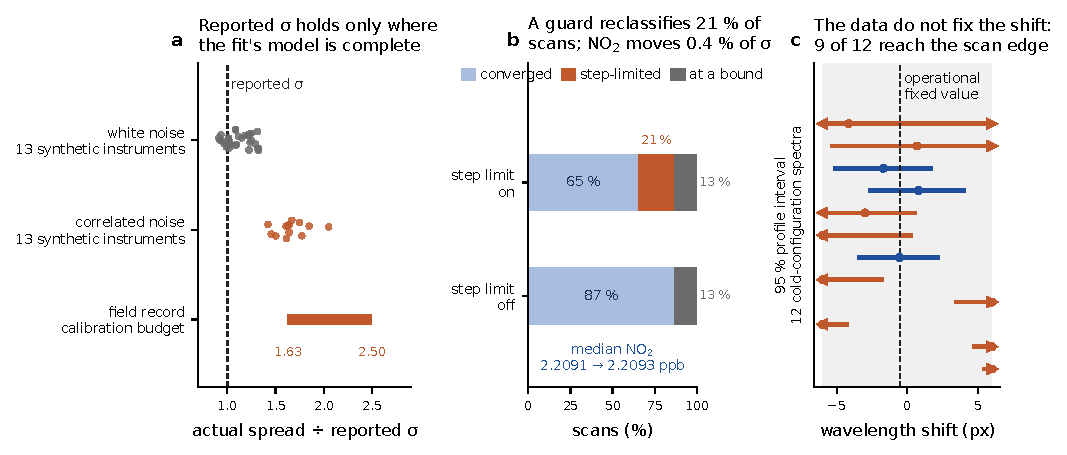
\includegraphics[width=\textwidth]{figures/fig01.pdf}
\caption{What a converged fit reports, and what the data support. \textbf{(a)} Spread of retrieved NO$_2$ over the
reported uncertainty. Grey: white noise, 30 cases over 13 synthetic instruments (line-shape width 0.5--2, window
0.7--1.3 and pixel dispersion 0.7--1.4 times nominal; signal-to-noise over a factor of 32; polynomial orders 2--6).
Orange: the same with AR(1) noise, $\rho = 0.5$. Bar: the field record, total uncertainty \fieldnum{1.63} (robust scale) to
\fieldnum{2.50} (standard deviation) times the fit-propagated $\sigma$ ($n = \fieldnum{8847}$ records of 60\,s). \textbf{(b)} Termination state
of \fieldnum{8446} operational scans, step limit on and off. \textbf{(c)} 95\,\% profile-likelihood
intervals of the cold-configuration shift for 12 spectra, scanned over $\pm6$\,px, with
$\mathrm{RSS}/\mathrm{RSS}_{\min} \le 1 + F_{0.95}(1, n-P)/(n-P)$, $n-P = 766$; arrows reach the scan edge;
dashed, the operational value, $-0.5$\,px.}
\label{fig:1}
\end{figure*}
